\documentclass[aspectratio=169,x11names]{beamer}
\usetheme{Pittsburgh}
\usepackage{xcolor}
\usepackage[utf8]{inputenc}
\usepackage[german]{babel}
\usepackage{amsmath}
\usepackage{amsfonts}
\usepackage{amssymb}
\usepackage{graphicx}
\usepackage{multicol}
\usepackage{wrapfig}
\usepackage{hyperref}
\usepackage{tikz}

\usetikzlibrary{shapes,arrows,chains}

\author{Jonas Betzendahl}
\title{Digital Self-Defense}

\beamertemplatenavigationsymbolsempty 

%src: https://tex.stackexchange.com/questions/34921/how-to-overlap-images-in-a-beamer-slide
\def\Put(#1,#2)#3{\leavevmode\makebox(0,0){\put(#1,#2){#3}}}

\begin{document}

%------------------------------------------------------------------------------------
\section{Introduction}

\begin{frame}
\begin{center}
\vfill
\huge Digital Self-Defence
\normalsize 
\smallskip
\smallskip

Levelling up your defence in a world\\ that is levelling up its offence.
\bigskip\bigskip

\large Jonas Betzendahl, M.Sc.\\
2019 -- 12 -- 05
\bigskip\bigskip

\href{https://twitter.com/lambdatotoro}{
\includegraphics[scale=0.125]{images/twitter_logo.png}}
\href{https://chaos.social/@lambdatotoro}{\includegraphics[scale=0.125]{images/mastodon_logo.png}}
\href{https://github.com/lambdaTotoro}{
\includegraphics[scale=0.125]{images/github_logo.png}}
\href{https://whispeer.de/en/user/jbetzend}{
\includegraphics[scale=0.125]{images/whispeer_logo.png}}

\texttt{@lambdaTotoro (@chaos.social)}
\end{center}
\end{frame}

\begin{frame}
\frametitle{Who am I?}
\end{frame}

%------------------------------------------------------------------------------------

\section{Technical Attacks}
\begin{frame}
\begin{center}
\huge Technical Attacks
\end{center}
\end{frame}

%------------------------------------------------------------------------------------

\section{Social Attacks}
\begin{frame}
\begin{center}
\huge Social Attacks
\end{center}
\end{frame}

\begin{frame}
\frametitle{How it works\dots}
\begin{minipage}[t]{0.49\textwidth}
\begin{center}
\vspace*{-15pt}
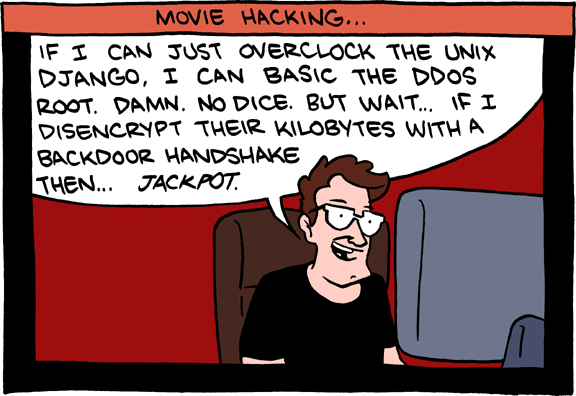
\includegraphics[width=\textwidth,keepaspectratio]{images/hackerman-1}
\end{center}
\end{minipage}
\begin{minipage}[t]{0.49\textwidth}
\begin{center}
\vspace*{15pt}
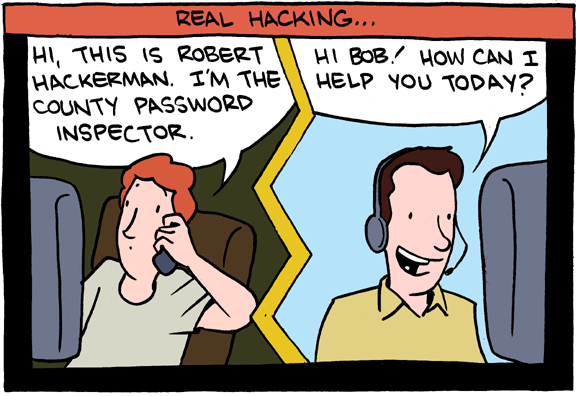
\includegraphics[width=\textwidth,keepaspectratio]{images/hackerman-2}
\end{center}
\end{minipage}
\end{frame}

%------------------------------------------------------------------------------------

\section{Conclusion}
\begin{frame}
\begin{center}
\huge Conclusion
\end{center}
\end{frame}

\begin{frame}
\frametitle{Recap}
\end{frame}

%------------------------------------------------------------------------------------

\section{End}

\begin{frame}
\frametitle{(Re)sources}
\footnotesize

\begin{itemize}
\item \emph{Coalition against Stalkerware}, \url{https://stopstalkerware.org/}
\end{itemize}

\end{frame}

\end{document}

